\begin{figure}[ht]
    \centering
    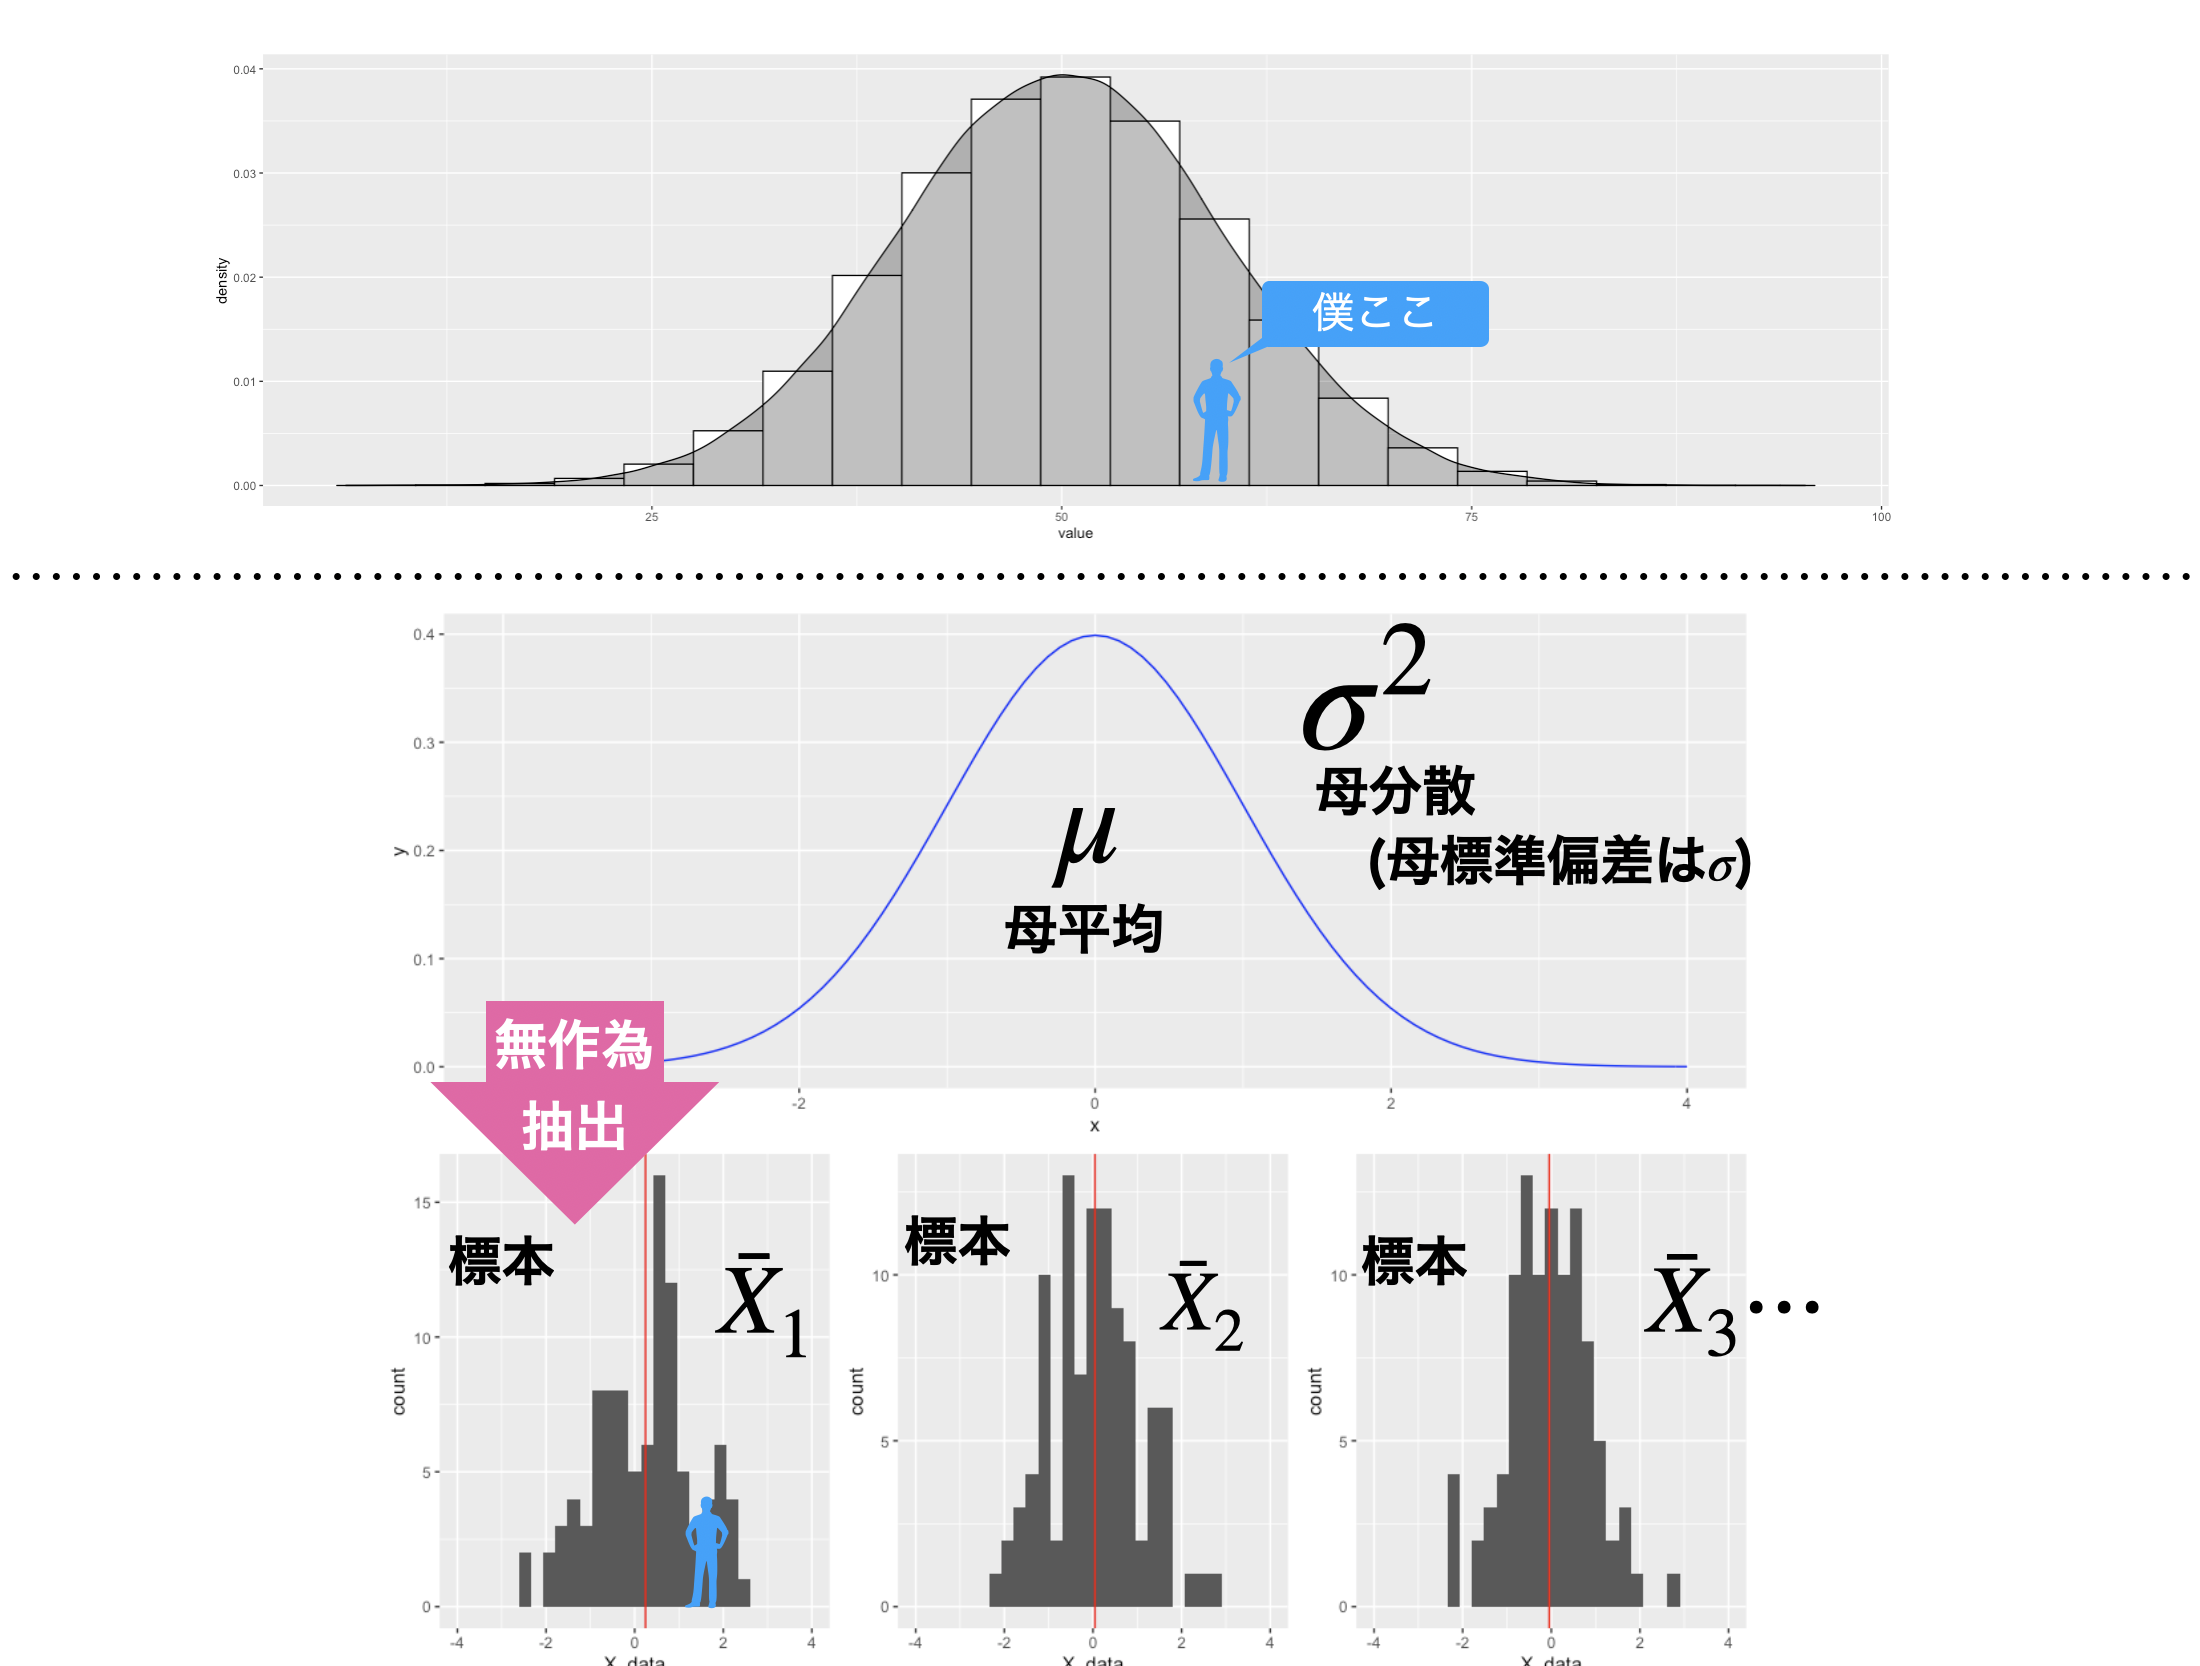
\includegraphics[keepaspectratio,height=0.6\linewidth]{../images/17_estimation_and_test/slide17_1.png}
    \caption{推測統計学の枠組みで考えることに注意。以前(セクション\ref{UsefulNormal})は上の図のように，推測するのではなくて母集団そのものの中に一個人のスコアを位置付けて，相対的な位置を考えよう，という話でした。今回は下のように，母集団が正規分布だと仮定して，そこから得られた標本のことについて考えています。個々のデータは標本の中にあります。また今回考えるのは標本統計量で，それが標本分布に従うのでした。}
    \label{fig::17_01}
\end{figure}
